\chapter{Eksperimentalno testiranje Belovih nejednakosti}


Eksperimenti za testiranje Belovih nejednakosti su izvedeni ve\' c 1960-ih i 1970-ih godina, a 2022. godine Nobelovu
nagradu su dobili Alen Aspekt (\textit{Alain Aspect}), D\v zon Klauzer (\textit{John Clauser}) i Anton Cajlinger (\textit{Anton Zeilinger}).

Oni su osmislili tri verzije eksperimenta u kojem se koriste polarizovani fotoni, umjesto raspada piona,
kako bi se testirale Belove nejednakosti. Da bi se isklju\v cilo "favorizovanje" određenih pravaca u eksperimentu, obje orijentacije su
postavljene kvazi-slu\v cajno nakon \v sto su fotoni ve\' c bili u letu.
Pokazalo se da su Belove nejednakosti u ovim eksperimentima naru\v sene, \v sto je zna\v cilo eksperimentalnu potvrdu
ispravnosti kvantne mehanike i propast "realizma" zbog nelokalnosti koju su eksperimenti potvrdili.
Ideja o nelokalnosti (u kontekstu superluminalnog uticaja) je svakako uznemiruju\' ca jer je toliko druga\v cija od onoga \v sto nam intuicija govori i ima neprihvatljive implikacije.
Prema specijalnoj teoriji relativnosti, postoje inercijalni sistemi u kojima se takav signal \v siri unazad u vremenu, pa bi efekti prethodili sopstvenim uzrocima - \v sto dovodi do
razli\v citih logi\v ckih anomalija.
Pitanje je da li su efekti posmatrani u ovim eksperimentima kauzalni, ili su dovoljno eteri\v cni da se izbjegne filozofski odgovor i da superluminalni uticaji u tom slu\v caju
dobiju novi interpretaciju.

Jedan od takvih primjera eteri\v cnih efekata bila bi sjenka bube koja preleti preko svjetlosnog snopa filmskog projektora (slika \ref{fig:bug_on_screen}). Udaljenost do ekrana mo\v ze biti proizvoljna, pa samim tim i brzina sjenke
mo\v ze biti proizvoljno velika, tako da mo\v zemo zamisliti scenario u kojem se sjenka bube kre\' ce brzinom ve\' com od brzine svjetlosti.
Ono \v sto ovdje moramo primjetiti je da sjenka ne nosi nikakvu energiju, niti prenosi bilo kakvu informaciju s jedne ta\v cke na drugu, tako da mi ne mo\v zemo iz ta\v cke $X$ prouzrokovati bilo
\v sta u ta\v cki $Y$ mainpulacijom prolazne sjenke.

\begin{figure}[H]
    \centering
    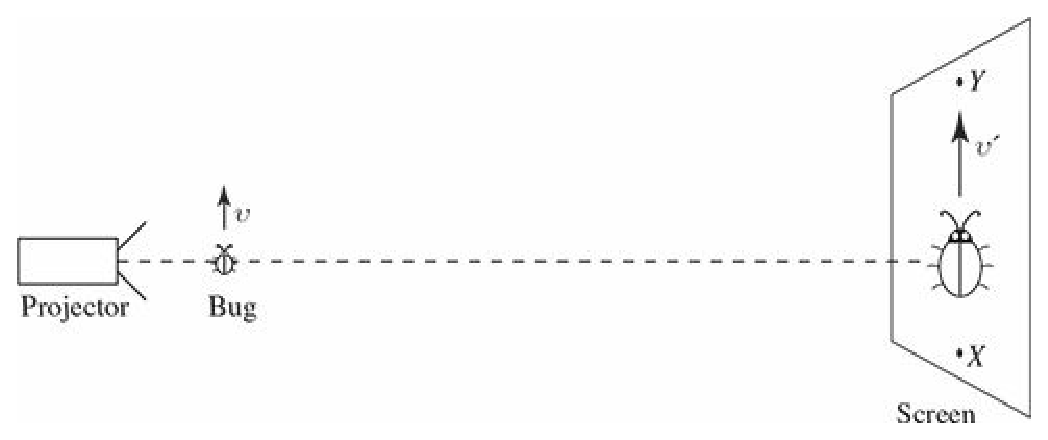
\includegraphics[width=0.75\textwidth]{figures/bug_on_screen.eps}
    \caption{Buba se kre\' ce brzinom $v$ preko svjetlosnog snopa filmskog projektora. U zavisnosti od udaljenosti platna, brzina $v^{'}$ mo\v ze biti proivoljno velika.}
    \label{fig:bug_on_screen}
\end{figure}

Hronolo\v ski, Klauzer je osmislio prvu verziju eksperimenta \v cija je 
su\v stina u slanju dva polarizovana spregnuta fotona, dobijena koriste\' ci atome Ca, u opozitnim smjerovima prema filterima kroz koje
\' ce foton ili pro\' ci ili ne\' ce, \v sto zavisi od ugla pod kojim je filter postavljen
i kako je foton polarizovan.

U momentu kreiranja para fotona ne mo\v zemo znati kakva im je polarizacija, ve\' c samo to da su im
polarizacije paralelne. To zna\v ci da ako su filteri postavljeni paralelno, u slu\v caju da jedan foton pro\dj e, vjerovatno\' ca da \' ce pro\' ci i drugi je $1$.
Ako je ugao izme\dj u filtera $\dfrac{\pi}{2}$ uvijek \' ce jedan foton pro\' ci, a drugi ne.

Zanimljivi efekti se vide ako se posmatraju uglovi filtera ba\v s izme\dj u $0$ i $\dfrac{\pi}{2}$. Tada rezultati variraju,
pa ponekad pro\dj u oba fotona, ponekad samo jedan, a u nekim slu\v cajevima nijedan.

Kada se uradi dosta mjerenja i zabilje\v ze se rezultati, mo\v ze se uo\v citi korelacija koja je mnogo ve\'ca nego kada bi
proces bio vo\dj en pod uticajem neke skrivene varijable pri \v cemu bi polarizacije fotona ve\'c bile predeterminisane u momentu njihove kreacije, a ne u trenutku mjerenja.

Ovaj eksperiment je unaprije\dj ena verzija misaonog Belovog eksperimenta, jer se koriste i detektori koji
detektuju fotone koji nisu uspjeli pro\'ci kroz filter, pa je samim tim eksperiment potpuniji i rezultat precizniji (slika \ref{fig:chsh_scheme}).
U svojoj sr\v zi ovaj eksperiment nosi korelacionu funkciju koja ima zadatak da modeluje odgovor na pitanje: "Koliko
\v cesto \'ce oba fotona pro\' ci kroz filtere, a koliko \v cesto samo jedan?", koja je ograni\v cena odozgo i predstavlja analognu formu
Belovih nejednakosti, zvanu CHSH nejednakost.

\begin{figure}
    \centering
    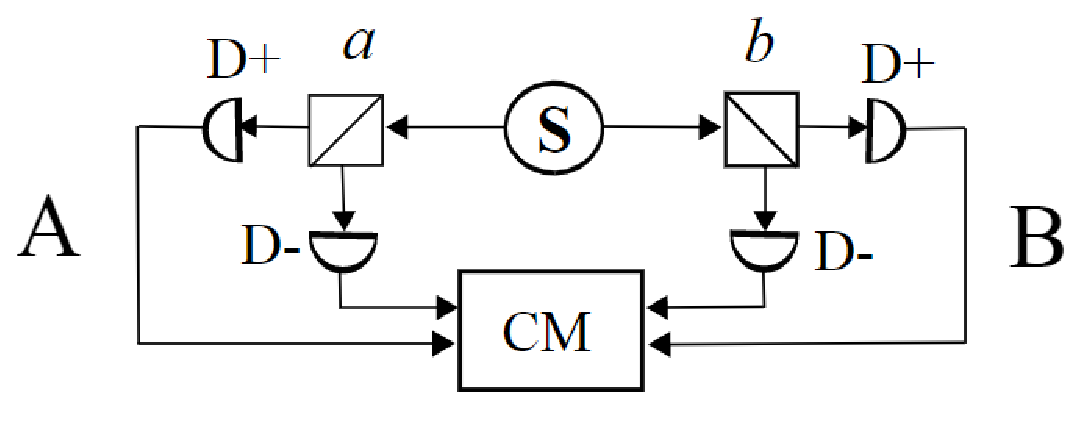
\includegraphics[width=0.75\textwidth]{figures/chsh_scheme.eps}
    \caption{Izvor \textit{S} emituje spregnute fotone koji potom odlaze u suprotnim smjerovima. U zavisnosti od njihove polarizacije i orijentacije filtera sti\'ci \' ce do  detektora $D_+$ ili $D_-$.
    Korelacija izme\dj u pojedina\v cnih mjerenja se mo\v ze izra\v cunati tako \v sto
    na\dj emo broj koji predstavlja odnos sume mjerenja pri kojima smo dobili rezultat da su oba fotona pro\v sla ili oba nisu pro\v sla kroz filter
    od koje smo oduzeli sumu mjerenja pri kojima je samo jedan od fotona pro\v sao kroz filter i ukupnog broja mjerenja, tj.
       $E(a,b) = N_{++} + N_{--} - (N_{+-} + N_{-+})/N$}
    \label{fig:chsh_scheme}
\end{figure}

Osim naru\v senja Belovih nejednakosti, novi potencijal za skladi\v stenje, preno\v senje i procesuiranje informacija je uvi\dj en sa novom verzijom eksperimenta, koju je osmislio Aspekt.

Konfiguracija eksperimenta je bila druga\v cija  u odnosu na Klauzerov u novom na\v cinu pobu\dj ivanja atoma tako da je frekvencija emitovanja
spregnutih fotona bila ve\'ca. Tako\dj e je kori\v sten kristal kvarca koji je slu\v zio za preusmjerenje fotona ka razli\v cito orijentisanim filterima.

Zanimljiv efekat se mogao vidjeti u slu\v caju kada se spregnuti par \v cestica (\v cestice $1$ i $2$) kre\' ce u suprotnim smjerovima i jedna od tih \v cestica nai\dj e na tre\'cu, slobodnu \v cesticu (\v cestica $3$).
U tom slu\v caju \v cestice $2$ i $3$ postaju spregnute, pri tome \v cestica $3$ gubi sve informacije o prethodnom stanju, ali se istovremeno to stanje "prepisuje" na \v cesticu $1$ koja
nikada nije ni do\v sla u kontakt sa \v cesticom $3$. Ovaj proces je poznat pod imenom \textit{kvatna teleportacija}.

Kvantna teleportacija je za sada jedini mehanizam kojim se nepoznato kvantno stanje (\textit{kvantna informacija}) mo\v ze u potpunosti prenijeti iz jednog u drugi sistem,
bez ikakvih gubitaka informacija. Nemogu\'ce je izmjeriti sve karakteristike sistema i poslati te informacije na drugu lokaciju, kako bi se
prvobitni sistem rekonstruisao, primarno zbog kolapsa talasne funkcije pri vr\v senju bilo kakvog mjerenja.

Nakon \v sto je kvantna teleportacija eksperimentalno pokazana, Cajlingerov eksperiment je dodao novu "dimenziju" eksperimentu i pokazao
mogu\' cnost sprezanja \v cestica koje su udaljene i nikada nisu do\v sle u kontakt.
Dva para (par \textit{A} i par \textit{B}) spregnutih \v cestica se emituju iz izvora. Nakon nekog vremena po jedna od \v cestica iz svakog para konvergiraju ka
ure\dj aju koji \' ce nekom transformacijom da u\v cini te dvije \v cestice spregnutima. Zbog kvantne teleportacije kvantne informacije preostalih
\v cestica \' ce se "prepisati" jedna na drugu i one \'ce postati spregnute iako nikada nisu do\v sle u kontakt.

